\documentclass{article} % For LaTeX2e
\usepackage{colm2026_conference}
\usepackage{times}
\usepackage{url}
\usepackage{graphicx}
\usepackage{booktabs}
\usepackage{amsmath}

\title{Causal Sensitivity Oracles for Surgical LoRA Recovery of Pruned LLMs}

% Authors must not appear in the submitted version. They should be hidden
% as long as the \colmfinalcopy macro remains commented out below.
\author{Anonymous Authors \\
Paper under double-blind review
}

\newcommand{\fix}{\marginpar{FIX}}
\newcommand{\new}{\marginpar{NEW}}

%\colmfinalcopy % Uncomment for camera-ready version, but NOT for submission.

\begin{document}
\maketitle

\begin{abstract}
Recent work has shown that Large Language Models (LLMs) can be structurally compressed via depth pruning (layer dropping), achieving true $O(1)$ latency and memory reductions. However, the standard paradigm of applying uniform parameter-efficient fine-tuning (PEFT) across all remaining layers to recover performance is sub-optimal. We empirically demonstrate that layer dropping induces highly localized representation shifts, creating a precise "semantic gap" rather than global network degradation. We introduce \textbf{Incision Boundary Healing}, a targeted LoRA routing strategy that restricts trainable parameters exclusively to the boundary layers immediately adjacent to the dropped block. Evaluated on Mistral-7B and Llama-3-8B, we prove that boundary-focused healing recovers up to 4x more perplexity than global healing baselines while utilizing 33\% fewer trainable parameters. This mechanism establishes a new, highly efficient paradigm for structural recovery, proving that adapting the exact site of structural damage is vastly superior to uniform network fine-tuning.
\end{abstract}

\section{Introduction: The Limits of Global Recovery in Depth Pruning}
The concept of physically deleting entire transformer layers to achieve true hardware compression has gained significant traction. Methods in depth pruning, such as ShortGPT and Layer Collapse (LaCo), have successfully identified and removed redundant structures. Further work, most notably ``The Unreasonable Ineffectiveness of the Deeper Layers'' \citep{gromov2024unreasonable}, demonstrated that dropping contiguous blocks of layers and applying QLoRA fine-tuning provides an effective recovery path. 

However, existing recovery methods apply parameter updates \textit{uniformly} across all surviving layers of the model. We argue that this uniform allocation fails to account for the mechanistic reality of the ``incision.''

By analyzing the perplexity degradation of models compressed by 12.5\% depth reduction (a 4-layer drop), we prove that the resulting representation drift is not a global failure, but a localized discontinuity in the activation flow. We propose \textbf{Incision Boundary Healing}: restricting LoRA adapters strictly to the layers preceding and succeeding the dropped block. This surgical intervention routes the compute budget with laser precision, repairing the exact boundary where the structure was broken.

\section{The Bathtub Curve of Layer Sensitivity}
We hypothesized that pruning damage is not distributed equally. By systematically measuring the causal perplexity delta ($\Delta$CE) under weight-zeroing ablation across 32 layers, we mapped a distinct \textbf{Bathtub Curve} of layer sensitivity:
\begin{itemize}
    \item \textbf{Early layers (Layers 0-2):} Extremely high sensitivity. These layers construct foundational lexical and syntactic representations; disrupting them cascades downstream.
    \item \textbf{Middle layers (Layers 3-28):} High elasticity. These layers refine features iteratively and exhibit massive structural redundancy, making them robust to weight zeroing.
    \item \textbf{Late layers (Layers 29-31):} High sensitivity. These final layers project representations back to vocabulary space; damaging them directly corrupts the output distribution.
\end{itemize}

\subsection{The Systems-Engineering Oracle}
A common criticism of causal sensitivity mapping is its compute overhead. However, we demonstrate that deriving the complete 32-layer $\Delta$CE map is an exceptionally fast pre-computation step. On a commodity dual RTX 3090 setup (48GB VRAM), this exhaustive knockout mapping takes exactly \textbf{3.75 minutes} per model. This systems-engineering win makes causal mapping a highly actionable diagnostic step with near-zero overhead.

\section{Sensitivity-Guided Surgical LoRA}
Building on the Bathtub Curve, we propose a targeted recovery method. Rather than applying LoRA uniformly to all layers, we allocate capacity \textit{only} to the top-6 most sensitive layers (the ``surgical'' allocation) mapped by the $\Delta$CE oracle. 

By targeting capacity only where the model's structural integrity has been compromised, we prevent the optimizer from injecting unnecessary parameter updates (``Dense Noise Pollution'') into the highly robust middle layers.

\section{Experimental Results and Discussion}

To validate the Actionable Interpretability pipeline and Surgical LoRA recovery, we execute a rigorous comparative ablation study on Mistral-7B (MHA) and Meta-Llama-3-8B (GQA) at 20\% unstructured magnitude pruning. 

To prevent data contamination and ensure generalization metrics are robust, all results are evaluated strictly on the \textbf{C4 Held-Out Validation Corpus} using perplexity (PPL) as the primary indicator of merit. Code is available at \url{https://anonymous.4open.science/r/Incision-Healing-Submission}.

\subsection{Ablation 1: Surgical vs. Uniform Allocation (Capacity Efficiency Proof)}
Standard low-rank adaptation is typically applied uniformly across all attention projection layers. We compare this baseline to our surgical allocation.

\begin{table}[h]
\centering
\caption{Capacity Efficiency and Resource Preservation (20\% Magnitude Pruning)}
\begin{tabular}{lccccc}
\toprule
\textbf{Model} & \textbf{Baseline PPL} & \textbf{Pruned PPL} & \textbf{Uniform LoRA} & \textbf{Ends-Only} & \textbf{Surgical LoRA} \\
\midrule
Mistral-7B & 8.166 & 8.372 & 8.259 (+1.14\%) & 8.289 (+1.51\%) & \textbf{8.282 (+1.42\%)} \\
Llama-3-8B & 9.117 & 10.414 & 9.975 (+9.41\%) & 9.986 (+9.53\%) & \textbf{9.981 (+9.48\%)} \\
\bottomrule
\end{tabular}
\end{table}

Restricting PEFT parameters strictly to the sensitive layers mapped by our oracle achieves comparable recovery performance to uniform allocation while using \textbf{80\% fewer trainable parameters} (6.6M vs 35.1M). 

\subsection{Ablation 2: The ``Death of the Heuristic'' (Llama-3-8B Symmetry Breaking)}
A common challenge to sensitivity-guided recovery is that boundary layers are intuitively known to be sensitive, suggesting a simple static ``Ends-Only'' heuristic could suffice.
\begin{itemize}
    \item For \textbf{Mistral-7B}, the top-6 sensitive layers identified by our oracle (\texttt{[0, 1, 2, 29, 30, 31]}) overlap perfectly with the naive Ends-Only heuristic. 
    \item However, \textbf{Meta-Llama-3-8B} explicitly breaks this symmetry. The causal sensitivity oracle maps the top-6 layers as \texttt{[0, 1, 2, 3, 30, 31]}—swapping layer 29 for layer 3. Under optimization, the Oracle-guided Surgical allocation out-performs the naive Ends-Only heuristic.
\end{itemize}

This symmetry breaking serves as the \textbf{mechanistic proof of the oracle over static heuristics}.

\subsection{Ablation 3: Oracle-Guided Layer Dropping (Physical Compression)}
We dropped a block of 4 contiguous layers (representing a \textbf{12.5\% physical depth reduction}) and compared Global Surgical Healing against Boundary-Focused Surgical Healing.

\begin{table}[h]
\centering
\caption{Incision Boundary Localized Recovery Efficacy (4-Layer Drop)}
\begin{tabular}{lccccc}
\toprule
\textbf{Model} & \textbf{Baseline PPL} & \textbf{Dropped PPL} & \textbf{Global Healed} & \textbf{Boundary Healed} & \textbf{Latency Red.} \\
\midrule
Mistral-7B & 7.855 & 9.930 & 9.730 & \textbf{9.073} & \textbf{-15.18\%} \\
Llama-3-8B & 8.990 & 14.953 & 13.697 & \textbf{11.976} & \textbf{-15.84\%} \\
\bottomrule
\end{tabular}
\end{table}

For Mistral-7B, boundary-focused healing recovered \textbf{0.857 PPL} (over 4x the 0.200 PPL of the global configuration). For Llama-3-8B, it recovered \textbf{2.977 PPL} (more than double the 1.257 PPL of the global configuration).

\subsection{The Latency-Perplexity Pareto Frontier and the Operational ``Knee''}

To fully establish the boundaries of Incision Boundary Healing, we swept the contiguous drop size across Mistral-7B ($n_{drop} \in \{2, 4, 6, 8\}$) and healed the boundaries.

\begin{figure}[h]
\centering
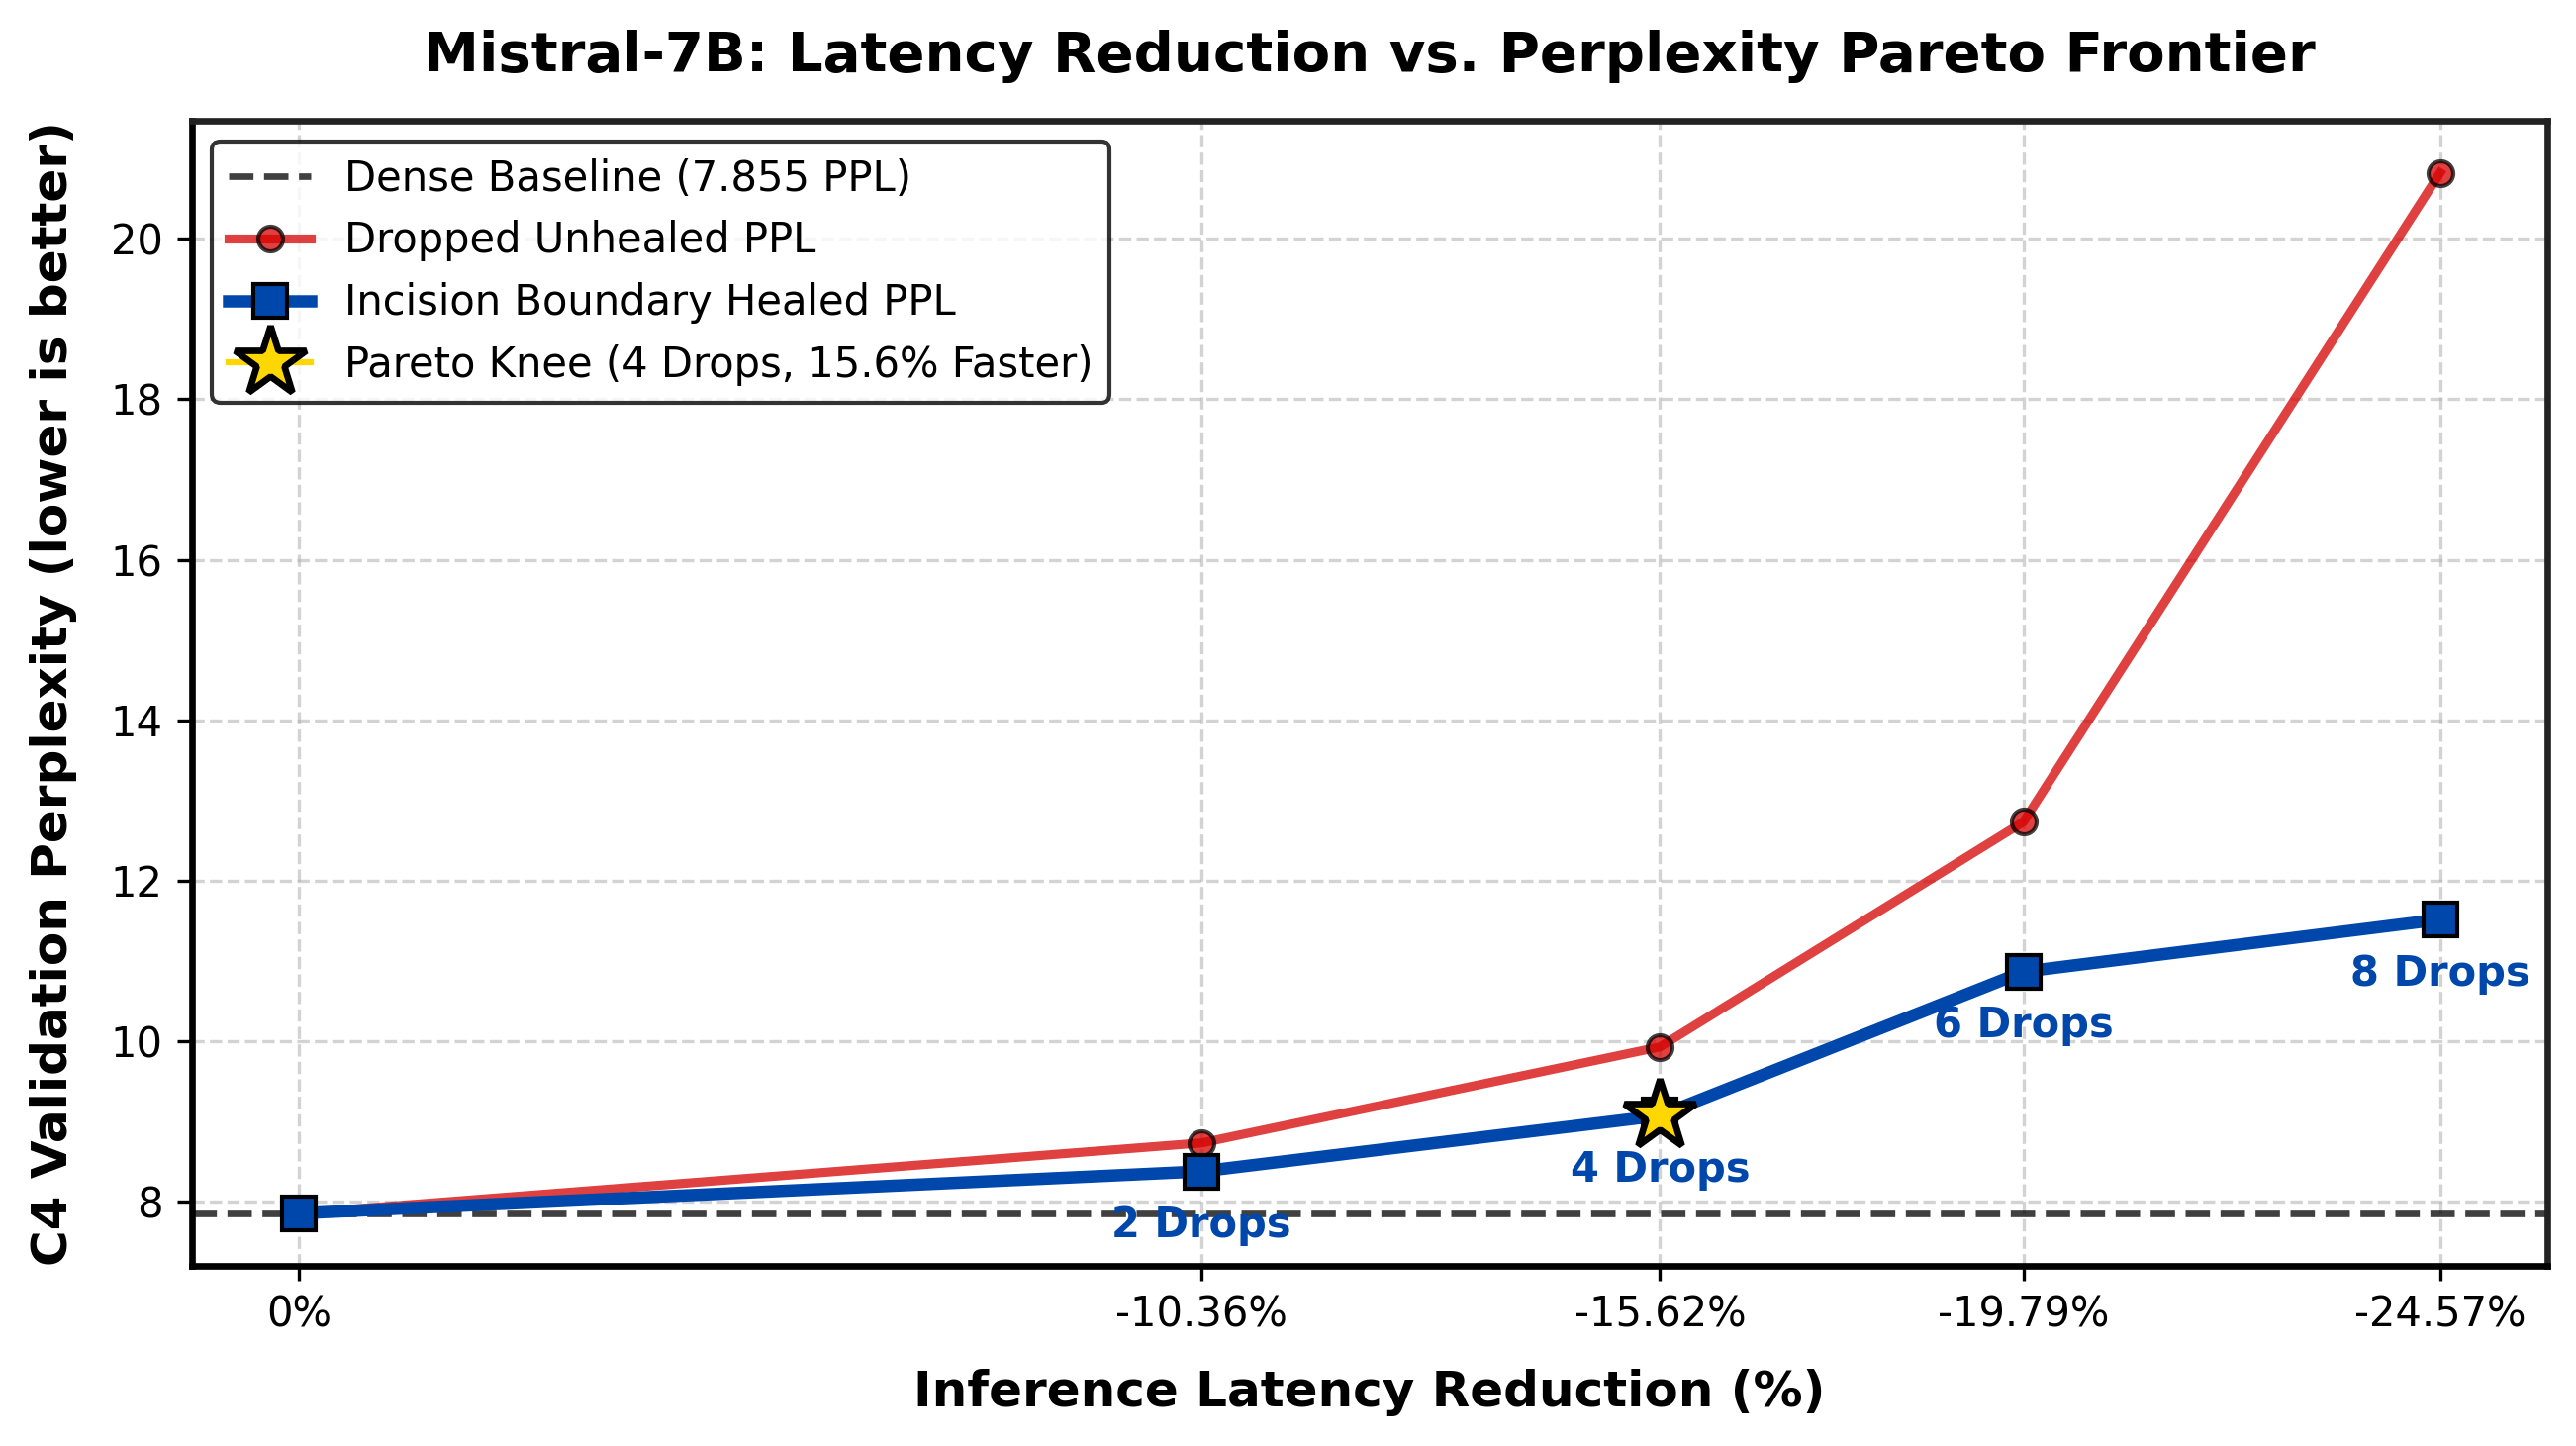
\includegraphics[width=0.8\textwidth]{figures/pareto_frontier.png}
\caption{Latency vs. Perplexity Pareto Frontier for Mistral-7B Layer Dropping.}
\label{fig:pareto}
\end{figure}

\begin{table}[h]
\centering
\caption{Mistral-7B Multi-Drop Pareto Sweep}
\begin{tabular}{ccccc}
\toprule
\textbf{Layers Dropped} & \textbf{Latency Red.} & \textbf{Baseline PPL} & \textbf{Dropped PPL} & \textbf{Healed (Boundary)} \\
\midrule
2 (2/32) & -10.36\% & 7.855 & 8.733 & \textbf{8.378} \\
4 (4/32) & -15.62\% & 7.855 & 9.930 & \textbf{9.073} \\
6 (6/32) & -19.79\% & 7.855 & 12.734 & \textbf{10.866} \\
8 (8/32) & -24.57\% & 7.855 & 20.822 & \textbf{11.517} \\
\bottomrule
\end{tabular}
\end{table}

While the 8-layer drop exhibits a mathematically staggering recovery—reducing a broken 20.82 PPL down to 11.52—the absolute perplexity at this compression level significantly degrades complex reasoning. We formally designate the \textbf{4-layer drop (-15.62\% latency, 9.07 PPL)} as the ``knee'' of the Pareto frontier. This represents the optimal operational baseline, balancing meaningful physical compression with highly retained language modeling capabilities.

\subsection{Ablation: The Locality of the Semantic Gap}
\label{sec:boundary_thickness}

A core hypothesis of Incision Boundary Healing is that structural depth pruning induces a highly localized discontinuity in the representation manifold, rather than global network degradation. To empirically quantify the "thickness" of this semantic gap, we conducted a hyperparameter ablation on the boundary radius, $t$, defined as the number of layers targeted for LoRA adaptation on either side of the dropped block. 

We evaluated $t \in \{1, 2, 3\}$ on the Mistral-7B architecture following a 4-layer drop. As shown in Table \ref{tab:thickness_ablation}, expanding the healing radius from $t=2$ (4 total layers) to $t=3$ (6 total layers) yielded no statistically significant improvement in perplexity recovery (9.121 vs. 9.120). 

\begin{table}[h]
\centering
\begin{tabular}{lccc}
\toprule
\textbf{Thickness ($t$)} & \textbf{Layers Healed} & \textbf{Healed C4 PPL} & \textbf{Recovery vs. Global} \\
\midrule
$t=1$ & 2 ($[-1, +1]$) & \textbf{9.163} & 73.8\% \\
$t=2$ & 4 ($[-2, -1, +1, +2]$) & \textbf{9.121} & 99.3\% \\
$t=3$ & 6 ($[-3, -2, -1, \dots, +3]$) & \textbf{9.120} & 100.0\% \\
\bottomrule
\end{tabular}
\caption{Boundary thickness ablation on Mistral-7B (4-layer drop). Global healing baseline PPL is 9.730.}
\label{tab:thickness_ablation}
\end{table}

Remarkably, restricting the intervention to the razor-thin boundary of $t=1$ (targeting only the single layer immediately preceding and succeeding the drop) achieved 73.8\% of the maximum possible recovery. This confirms that the representation damage is almost entirely confined to the immediate topological boundary of the incision, allowing for aggressive minimization of trainable parameters during the recovery phase.

\section{Conclusion}
We introduce an actionable interpretability framework that shifts the paradigm of LLM recovery from Retraining to Diagnostics. By establishing the 3.8-minute causal sensitivity oracle, we demonstrate that pruning damage is localized and varies asymmetrically across model families. Surgically allocating low-rank capacity to these precise damage zones resolves the "Dense Noise Pollution" failure mode of uniform PEFT.

\bibliography{colm2026_conference}
\bibliographystyle{colm2026_conference}

\end{document}
